\documentclass[11pt,a4paper]{article}

\usepackage[utf8]{inputenc}
\usepackage[T1]{fontenc}
\usepackage[spanish,es-tabla]{babel}
\usepackage{amsmath,amssymb,amsfonts}
\usepackage{graphicx}
\usepackage{geometry}
\usepackage{booktabs}
\usepackage{xcolor}
\usepackage{float}
\usepackage{hyperref}
\usepackage{enumitem}
\usepackage{array}
\usepackage{microtype}

\geometry{
    top=2.5cm,
    bottom=2.5cm,
    left=2.5cm,
    right=2.5cm
}

\hypersetup{
    colorlinks=true,
    linkcolor=blue!80!black,
    citecolor=blue!80!black,
    urlcolor=blue!80!black
}

\title{
    \vspace{-1.5cm}
    \textbf{Informe de Proyecto: Inteligencia Artificial} \\[0.3cm]
    \Large \textbf{Sistema Híbrido de Inteligencia Artificial para la Clasificación de Calidad del Vino Tinto: Minería de Reglas (PRISM y Apriori), Inferencia Difusa Mamdani y Calibración Evolutiva con Algoritmos Genéticos}
}

\author{
    \textbf{Asignatura:} Inteligencia Artificial / Computación Evolutiva \\[0.1cm]
    \textbf{Proyecto Final Integrador} \\[0.1cm]
    \textit{Facultad de Ingeniería -- Carrera de Ingeniería de Sistemas}
}

\date{\today}

\begin{document}

\maketitle

\begin{abstract}
En este trabajo se presenta el diseño, fundamentación matemática e implementación desde cero de un sistema híbrido de inteligencia artificial explicable (\textit{Explainable AI - XAI}) para la predicción de la calidad del vino tinto a partir del conjunto de datos fisicoquímicos \textit{Wine Quality Dataset} (1,599 instancias). Los clasificadores basados en reglas lógicas convencionales presentan el severo dilema de las fronteras rígidas (\textit{boundary problem}): variaciones infinitesimales en variables continuas provocan abstenciones o saltos discretos artificiales, limitando la cobertura y robustez del modelo. Para resolver esta problemática sin recurrir a modelos de ``caja negra'' opacos (redes neuronales o ensambles complejos), implementamos una metodología progresiva de tres fases: (1) \textbf{Minería dual de conocimiento desde cero} combinando inducción modular estricta (\textbf{PRISM}, 16 reglas) y reglas de asociación (\textbf{Apriori}, 1,031 reglas filtradas) sobre la totalidad de las \textbf{11 variables fisicoquímicas}, consolidando una base integrada de 26 reglas unificadas; (2) \textbf{Sistema de Inferencia Difusa Mamdani continuo}, que transforma los términos lingüísticos en funciones de pertenencia continuas híbridas (Trapezoidales y Triangulares) con agregación continua y defuzzificación por Centroide cuantitativo (CoG en $[0, 10]$); y (3) \textbf{Calibración simultánea mediante Algoritmo Genético (DEAP / NumPy)} que optimiza un cromosoma mixto de 59 genes (33 puntos de corte $a_i < b_i < c_i$ y 26 pesos de activación de reglas) mediante una función de aptitud multi-criterio ponderada ($\text{Fitness} = 0.70\cdot\text{F1\_Macro} + 0.20\cdot\text{Cob} - 0.10\cdot\text{Comp}$). En el conjunto de prueba independiente ($N=320$, 20\% estratificado), el modelo optimizado alcanzó un \textbf{60.31\% de Exactitud}, un \textbf{F1-Macro de 0.5647} (+9.73 puntos porcentuales sobre el baseline discreto de 0.4674), una \textbf{Cobertura del 99.38\%} (+19.69 puntos porcentuales) y ejecutó una \textbf{poda automática del 38.5\% de reglas redundantes} (reduciendo de 26 a 16 reglas activas). Finalmente, el sistema se integró en una aplicación web interactiva que expone en tiempo real las trazas de inferencia y la justificación química de cada decisión.
\end{abstract}

\vspace{0.3cm}
\noindent\textbf{Palabras clave:} PRISM, Apriori, Lógica Difusa Mamdani, Algoritmos Genéticos, Optimización Multi-criterio, Cromosoma Mixto, Wine Quality, Inteligencia Artificial Explicable (XAI).

\vspace{0.4cm}

% =============================================================================
\section{Introducción y Planteamiento del Problema}
% =============================================================================

El control de calidad en la industria enológica representa un desafío crítico de alta complejidad bioquímica. Tradicionalmente, la evaluación de la calidad organoléptica del vino depende de paneles de catadores expertos. Si bien la cata sensorial provee un criterio holístico insustituible, está sujeta a variabilidad humana, fatiga sensorial, sesgos subjetivos y elevados costos operativos. En consecuencia, el modelado computacional que predice la calidad a partir de parámetros fisicoquímicos obtenidos en laboratorio ofrece un soporte de decisión cuantitativo invaluable.

El dataset de referencia internacional para este propósito es el \textit{Wine Quality Dataset} (\cite{cortez2009modeling}), proveniente del repositorio UCI Machine Learning. Contiene 1,599 muestras de vino tinto (\textit{Vinho Verde}), caracterizadas por 11 propiedades fisicoquímicas cuantitativas continuas y una calificación sensorial discreta en la escala de 0 a 10.

Al abordar este problema desde el paradigma de la minería de datos y el aprendizaje automático, surge un dilema fundamental:
\begin{enumerate}
    \item Los modelos de alta capacidad predictiva como las Redes Neuronales Profundas, Support Vector Machines o ensambles de Gradient Boosting operan como \textbf{cajas negras}. Carecen de una semántica accesible para el enólogo, quien requiere comprender qué balance de acidez, alcohol o compuestos sulfurados determina el fallo o éxito de un lote.
    \item Los modelos interpretables basados en reglas lógicas booleanas convencionales sufren del \textbf{problema de frontera} (\textit{boundary problem}). Si se discretiza el alcohol mediante un umbral rígido en $10.80\%$, una muestra con $10.79\%$ será clasificada como ``Media'' y no activará ninguna regla de vinos de ``Alta'' calidad, perdiendo continuidad física y desplomando la capacidad de generalización ante datos no vistos.
\end{enumerate}

Para superar esta limitación sin sacrificar la transparencia explicativa, este proyecto formula una arquitectura híbrida en tres fases consecutivas:
\begin{itemize}[noitemsep]
    \item \textbf{Fase 1 (Modelo Base Discreto):} Descubrimiento inductivo y asociativo de reglas mediante implementaciones desde cero de los algoritmos **PRISM** y **Apriori** sobre las 11 variables fisicoquímicas discretizadas por cuantiles empíricos.
    \item \textbf{Fase 2 (Sistema Difuso Mamdani Inicial - Pre-AG):} Fuzzificación continua de todas las variables mediante funciones de pertenencia híbridas trapezoidales-triangulares, inferencia difusa con operador MIN, agregación MAX y defuzzificación por Centroide continuo (CoG).
    \item \textbf{Fase 3 (Sistema Difuso Optimizado - Post-AG):} Ajuste fino y simultáneo de la geometría de los conjuntos difusos y selección/poda de la base de reglas mediante un Algoritmo Genético con cromosoma mixto de 59 genes y función de aptitud multi-criterio.
\end{itemize}

% =============================================================================
\section{Fase 1 a 4: Preparación, Análisis Estadístico y Discretización}
% =============================================================================

\subsection{Conservación Integral de las 11 Variables Fisicoquímicas}
A diferencia de aproximaciones reduccionistas que descartan arbitrariamente variables químicas, este sistema conserva la totalidad de las **11 características predictoras** continuas del vino tinto:
\begin{enumerate}[noitemsep]
    \item \textbf{Acidez Fija (\textit{fixed acidity}, $\text{g/dm}^3$ ácido tartárico):} Responsable de la estructura y frescura inicial en paladar.
    \item \textbf{Acidez Volátil (\textit{volatile acidity}, $\text{g/dm}^3$ ácido acético):} Principal marcador de deterioro bacteriano; concentraciones elevadas producen notas avinagradas.
    \item \textbf{Ácido Cítrico (\textit{citric acid}, $\text{g/dm}^3$):} Aporta frescura y contribuye a la preservación del color.
    \item \textbf{Azúcar Residual (\textit{residual sugar}, $\text{g/dm}^3$):} Cantidad remanente tras la fermentación; determina el dulzor y balance tánico.
    \item \textbf{Cloruros (\textit{chlorides}, $\text{g/dm}^3$ NaCl):} Contenido mineral salino; influye en el cuerpo y redondez.
    \item \textbf{Dióxido de Azufre Libre (\textit{free sulfur dioxide}, $\text{mg/dm}^3$):} Fracción activa de $\text{SO}_2$ que previene la oxidación y contaminación microbiana.
    \item \textbf{Dióxido de Azufre Total (\textit{total sulfur dioxide}, $\text{mg/dm}^3$):} Suma de $\text{SO}_2$ libre y ligado; valores excesivos apagan los aromas frutales.
    \item \textbf{Densidad (\textit{density}, $\text{g/cm}^3$):} Correlacionada directamente con el contenido alcohólico y azúcares disueltos.
    \item \textbf{pH:} Nivel de disociación ácida global; condiciona la estabilidad biológica y la longevidad del vino.
    \item \textbf{Sulfatos (\textit{sulphates}, $\text{g/dm}^3$ $\text{K}_2\text{SO}_4$):} Coadyuvante antioxidante que potencia la acción del dióxido de azufre.
    \item \textbf{Alcohol (\textit{alcohol}, \% vol.):} Grado volumétrico etílico; aporta calidez, textura y preserva los aromas.
\end{enumerate}

\subsection{Categorización de la Variable Objetivo}
La calificación sensorial original se distribuye entre las puntuaciones 3 y 8 con un notable desbalance de clases (las notas extremas 3 y 8 representan menos del 5\% acumulado). Siguiendo las directrices académicas, la variable se proyectó a tres categorías cualitativas:
\begin{itemize}[noitemsep]
    \item \textbf{BAJA (notas 3, 4 y 5):} 744 muestras (46.53\%). Vinos defectuosos o desequilibrados.
    \item \textbf{MEDIA (nota 6):} 638 muestras (39.90\%). Vinos comerciales estándares.
    \item \textbf{ALTA (notas 7 y 8):} 217 muestras (13.57\%). Vinos de calidad superior o gran reserva.
\end{itemize}

\subsection{Partición Estratificada y Discretización por Cuantiles (Terciles)}
Para impedir la fuga de información (\textit{data leakage}), los parámetros de discretización se calcularon exclusivamente sobre el conjunto de entrenamiento (80\%, 1,279 vinos) mediante cuantiles empíricos de igual frecuencia (Equal-Frequency: 33\% Bajo, 33\% Medio, 33\% Alto), y se congelaron para transformar el conjunto de prueba (20\%, 320 vinos). La Tabla \ref{tab:estadisticas_cortes} resume las estadísticas descriptivas y los puntos de corte empíricos iniciales.

\begin{table}[H]
\centering
\caption{Estadísticas descriptivas y puntos de corte iniciales por terciles ($P_{33}, P_{66}$) en entrenamiento ($N=1,279$).}
\label{tab:estadisticas_cortes}
\small
\begin{tabular}{lcccccc}
\toprule
\textbf{Variable Fisicoquímica} & \textbf{Mínimo} & \textbf{Corte $a$ ($P_{33}$)} & \textbf{Mediana ($P_{50}$)} & \textbf{Corte $b$ ($P_{66}$)} & \textbf{Máximo} & \textbf{Asimetría} \\
\midrule
Fixed Acidity ($\text{g/dm}^3$) & 4.60 & 7.10 & 7.90 & 9.20 & 15.90 & 0.98 \\
Volatile Acidity ($\text{g/dm}^3$) & 0.12 & 0.39 & 0.52 & 0.64 & 1.58 & 0.67 \\
Citric Acid ($\text{g/dm}^3$) & 0.00 & 0.09 & 0.26 & 0.42 & 1.00 & 0.32 \\
Residual Sugar ($\text{g/dm}^3$) & 0.90 & 1.90 & 2.20 & 2.60 & 15.50 & 4.54 \\
Chlorides ($\text{g/dm}^3$) & 0.012 & 0.070 & 0.079 & 0.090 & 0.611 & 5.68 \\
Free Sulfur Dioxide ($\text{mg/dm}^3$) & 1.0 & 7.0 & 14.0 & 21.0 & 72.0 & 1.25 \\
Total Sulfur Dioxide ($\text{mg/dm}^3$) & 6.0 & 22.0 & 38.0 & 62.0 & 289.0 & 1.52 \\
Density ($\text{g/cm}^3$) & 0.9901 & 0.9956 & 0.9968 & 0.9978 & 1.0037 & 0.07 \\
pH & 2.74 & 3.21 & 3.31 & 3.40 & 4.01 & 0.19 \\
Sulphates ($\text{g/dm}^3$) & 0.33 & 0.55 & 0.62 & 0.73 & 2.00 & 2.43 \\
Alcohol (\% vol.) & 8.40 & 9.50 & 10.20 & 11.10 & 14.90 & 0.86 \\
\bottomrule
\end{tabular}
\end{table}

% =============================================================================
\section{Minería de Reglas desde Cero: PRISM y Apriori (Fases 5, 6 y 7)}
% =============================================================================

\subsection{Fase 5: Algoritmo Inductivo PRISM (Cendrowska, 1987)}
Se implementó el algoritmo PRISM íntegramente desde cero sin dependencias externas. A diferencia de C4.5 que construye árboles particionando el espacio completo, PRISM opera mediante \textbf{recubrimiento secuencial} (\textit{separate-and-conquer}), descubriendo reglas modulares ortogonales por cada clase objetivo $C \in \{\text{Alta}, \text{Baja}, \text{Media}\}$.

En cada iteración voraz sobre el conjunto de instancias activas $S$, PRISM selecciona el par $(\text{Variable}_i = \text{Valor}_j)$ que maximiza la precisión condicional empírica:
\begin{equation}
p(C \mid \text{Var}_i = \text{Val}_j) = \frac{|\{x \in S \mid \text{Var}_i(x) = \text{Val}_j \land \text{Clase}(x) = C\}|}{|\{x \in S \mid \text{Var}_i(x) = \text{Val}_j\}|}
\end{equation}
En caso de empate en precisión, el criterio de desempate selecciona la condición con mayor soporte de positivos locales, y subsidiariamente con mayor cobertura total.

Con umbrales de $\text{Precisión Mínima} = 0.60$, $\text{Instancias Mínimas} = 5$ y longitud máxima de 4 condiciones, PRISM descubrió **16 reglas modulares** (1 para clase Alta, 4 para Baja y 11 para Media), alcanzando un 63.10\% de exactitud en Train y un 57.19\% en Test.

\subsection{Fase 6: Algoritmo de Reglas de Asociación Apriori (Agrawal \& Srikant, 1994)}
Para enriquecer la base de conocimiento y cubrir correlaciones complejas no capturadas por el enfoque voraz de PRISM, se implementó desde cero el algoritmo **Apriori**:
\begin{enumerate}[noitemsep]
    \item \textbf{Generación de Candidatos $C_k$:} A partir de los itemsets frecuentes $L_{k-1}$ mediante unión por prefijo lexicográfico ($(k-1)$-prefijo común).
    \item \textbf{Poda Apriori (\textit{Pruning}):} Eliminación a priori de candidatos si alguno de sus subconjuntos de tamaño $k-1$ no pertenece a $L_{k-1}$.
    \item \textbf{Filtro Estricto Hacia la Variable Objetivo:} De las asociaciones extraídas, se filtraron exclusivamente aquellas donde el consecuente fuera una etiqueta válida de calidad: $\text{Antecedentes} \implies \text{calidad\_categoria} \in \{\text{Alta}, \text{Media}, \text{Baja}\}$.
\end{enumerate}

Aplicando umbrales de $\text{Soporte} \ge 0.02$, $\text{Confianza} \ge 0.60$ y $\text{Lift} > 1.20$, el motor analizó 12,678 itemsets frecuentes y extrajo **1,031 reglas de asociación** orientadas a la calidad (con valores de Lift de hasta $4.6155$).

\subsection{Fase 7: Integración y Selección de la Base Unificada de Reglas}
Para consolidar una base interpretable y parsimoniosa, se fusionó la estructura de ambos algoritmos bajo un esquema unificado:
\begin{enumerate}[noitemsep]
    \item Se incorporaron las **16 reglas modulares de PRISM** como núcleo clasificador principal.
    \item Se complementó con las mejores reglas de **Apriori** ordenadas descendentemente por Lift y Confianza, aplicando un límite de hasta 5 reglas asociativas no redundantes por clase.
    \item Se eliminaron duplicados exactos mediante comparación de firmas lexicográficas $\text{Antecedentes} \to \text{Consecuente}$.
\end{enumerate}

La base integrada resultante quedó compuesta por **26 reglas unificadas** (16 provenientes de PRISM y 10 de Apriori). La Tabla \ref{tab:reglas_muestra} expone una muestra de las reglas más influyentes.

\begin{table}[H]
\centering
\caption{Muestra representativa de la base de 26 reglas unificadas integradas (PRISM + Apriori).}
\label{tab:reglas_muestra}
\small
\begin{tabular}{cclcccc}
\toprule
\textbf{ID} & \textbf{Origen} & \textbf{Regla Lingüística (Antecedente $\to$ Consecuente)} & \textbf{Prec./Conf.} & \textbf{Soporte} & \textbf{Lift} \\
\midrule
$R_{1}$ & PRISM & SI alcohol=Alto $\land$ vol\_acidity=Bajo $\land$ tot\_sulfur=Bajo $\land$ sulphates=Alto $\to$ ALTA & 78.6\% & 1.7\% & 1.50 \\
$R_{2}$ & PRISM & SI alcohol=Bajo $\land$ volatile acidity=Alto $\to$ BAJA & 76.5\% & 13.6\% & 1.50 \\
$R_{3}$ & PRISM & SI volatile acidity=Alto $\land$ total sulfur dioxide=Alto $\to$ BAJA & 80.9\% & 8.9\% & 1.50 \\
$R_{6}$ & PRISM & SI alcohol=Alto $\land$ free sulfur dioxide=Alto $\to$ MEDIA & 61.8\% & 9.6\% & 1.50 \\
$R_{17}$ & Apriori & SI alcohol=Alto $\land$ density=Bajo $\land$ fixed acidity=Alto $\to$ ALTA & 62.8\% & 2.1\% & 4.62 \\
$R_{18}$ & Apriori & SI free sulfur=Alto $\land$ pH=Bajo $\land$ volatile acidity=Alto $\to$ BAJA & 94.7\% & 2.8\% & 2.04 \\
$R_{22}$ & Apriori & SI alcohol=Bajo $\land$ sulphates=Bajo $\land$ total sulfur dioxide=Bajo $\to$ BAJA & 92.3\% & 3.8\% & 1.98 \\
$R_{23}$ & Apriori & SI density=Bajo $\land$ sulphates=Medio $\land$ total sulfur dioxide=Bajo $\to$ MEDIA & 77.5\% & 2.4\% & 1.94 \\
\bottomrule
\end{tabular}
\end{table}

\subsection{Modelo Base Discreto (Baseline - Fase 1)}
El clasificador discreto evalúa las reglas en formato booleano mediante votación ponderada por confianza ($\text{Voto}_c = \sum_{r \in \text{Activas}(c)} w_r \cdot \text{Confianza}_r$). En el conjunto de prueba ($N=320$), el Baseline obtuvo:
\begin{equation*}
\text{Exactitud} = 57.50\%, \quad \text{F1-Macro} = 0.4674, \quad \text{Cobertura} = 79.69\%
\end{equation*}
Un 20.31\% de las muestras de prueba no activó ninguna regla y debió recurrir a la clase mayoritaria por abstención, evidenciando empíricamente la severidad del \textit{boundary problem}.

% =============================================================================
\section{Fase 8 y 9: Sistema de Inferencia Difusa Mamdani Continuo}
% =============================================================================

Para proporcionar suavizado matemático continuo, se diseñó un motor de lógica difusa tipo Mamdani (\cite{mamdani1975experiment}) vectorizado en NumPy sobre las 11 variables continuas.

\subsection{Funciones de Pertenencia Híbridas (Trapezoidal-Triangular)}
Para cada una de las 11 variables $x_i$, se definen tres conjuntos difusos utilizando los puntos de corte paramétricos $[a_i, b_i, c_i]$ con la restricción de orden estricta $\min_i \le a_i < b_i < c_i \le \max_i$:
\begin{enumerate}
    \item \textbf{Conjunto ``Bajo'' ($\mu_{\text{Bajo}}$):} Función trapezoidal con hombro izquierdo abierto:
    \begin{equation}
    \mu_{\text{Bajo}}(x; a, b) = \begin{cases}
    1.0, & x \le a \\
    \dfrac{b - x}{b - a}, & a < x < b \\
    0.0, & x \ge b
    \end{cases}
    \end{equation}
    \item \textbf{Conjunto ``Medio'' ($\mu_{\text{Medio}}$):} Función triangular simétrica centrada en $b$:
    \begin{equation}
    \mu_{\text{Medio}}(x; a, b, c) = \begin{cases}
    \dfrac{x - a}{b - a}, & a < x \le b \\
    \dfrac{c - x}{c - b}, & b < x < c \\
    0.0, & \text{en otro caso}
    \end{cases}
    \end{equation}
    \item \textbf{Conjunto ``Alto'' ($\mu_{\text{Alto}}$):} Función trapezoidal con hombro derecho abierto:
    \begin{equation}
    \mu_{\text{Alto}}(x; b, c) = \begin{cases}
    0.0, & x \le b \\
    \dfrac{x - b}{c - b}, & b < x < c \\
    1.0, & x \ge c
    \end{cases}
    \end{equation}
\end{enumerate}

\subsection{Motor de Inferencia y Defuzzificación por Centroide Continuo}
El flujo de inferencia opera en cuatro etapas analíticas:
\begin{enumerate}
    \item \textbf{Fuzzificación Vectorizada:} Mapea las 11 entradas continuas a una matriz de grados de pertenencia $\mu_{i,j}(x) \in [0.0, 1.0]$.
    \item \textbf{Fuerza de Disparo de Regla ($\alpha_k$):} Combina los antecedentes con la T-norma de Gödel (operador MIN) multiplicada por el peso $w_k \in [0.0, 1.0]$ de la regla:
    \begin{equation}
    \alpha_k = w_k \cdot \min_{(v, l) \in \text{Antecedentes}_k} \mu_{v, l}(x)
    \end{equation}
    \item \textbf{Agregación Difusa Mamdani:} Se calcula el corte máximo por clase $c \in \{\text{Baja}, \text{Media}, \text{Alta}\}$:
    \begin{equation}
    \alpha_c = \max_{k \mid \text{Consecuente}_k = c} \alpha_k
    \end{equation}
    Sobre el universo de discurso continuo de calidad $Z = [0.0, 10.0]$ (discretizado con paso $\Delta z = 0.1$), la curva agregada global se compone mediante la T-conorma MAX:
    \begin{equation}
    \mu_{\text{agregada}}(z) = \max \Big( \min(\alpha_{\text{Baja}}, \mu_{\text{Salida,Baja}}(z)), \min(\alpha_{\text{Media}}, \mu_{\text{Salida,Media}}(z)), \min(\alpha_{\text{Alta}}, \mu_{\text{Salida,Alta}}(z)) \Big)
    \end{equation}
    donde los conjuntos de salida lingüística están parametrizados como: $\text{Baja} = [0, 0, 4.0, 5.5]$ (trapezoidal), $\text{Media} = [4.5, 6.0, 7.2]$ (triangular) y $\text{Alta} = [6.5, 7.8, 10, 10]$ (trapezoidal).
    \item \textbf{Defuzzificación por Centroide de Gravedad (CoG):}
    \begin{equation}
    z^* = \frac{\int_{0}^{10} z \cdot \mu_{\text{agregada}}(z) \, dz}{\int_{0}^{10} \mu_{\text{agregada}}(z) \, dz} \approx \frac{\sum_m z_m \cdot \mu_{\text{agregada}}(z_m)}{\sum_m \mu_{\text{agregada}}(z_m)}
    \end{equation}
    El centroide cuantitativo continuo $z^* \in [0, 10]$ se discretiza en la clase final mediante umbrales óptimos:
    \begin{equation}
    \text{Predicción}(z^*) = \begin{cases}
    \text{BAJA}, & \text{si } z^* < 5.30 \\
    \text{ALTA}, & \text{si } z^* \ge 6.60 \\
    \text{MEDIA}, & \text{en otro caso } (5.30 \le z^* < 6.60)
    \end{cases}
    \end{equation}
\end{enumerate}

% =============================================================================
\section{Fases 10 y 11: Optimización con Algoritmos Genéticos (DEAP)}
% =============================================================================

Los cortes por cuantiles son una referencia empírica general, pero no maximizan la separabilidad entre clases ni distinguen la relevancia relativa entre reglas. Para resolver esta optimización no lineal de alta dimensionalidad, se diseñó un Algoritmo Genético continuo utilizando la librería **DEAP** (\textit{Distributed Evolutionary Algorithms in Python}) acoplada con matrices NumPy.

\subsection{Cromosoma Mixto de 59 Genes}
Cada individuo $\boldsymbol{\theta}$ codifica una solución candidata completa mediante un vector de longitud fija:
\begin{equation}
\boldsymbol{\theta} = \big[ \underbrace{a_1, b_1, c_1, \dots, a_{11}, b_{11}, c_{11}}_{\text{Genes 0..32: 33 puntos de corte de MFs}} \;\big\vert\; \underbrace{w_1, w_2, \dots, w_{26}}_{\text{Genes 33..58: 26 pesos de reglas en } [0.0, 1.0]} \big]
\end{equation}

\subsection{Operador de Reparación y Factibilidad Estricta}
Las mutaciones y cruces pueden violar la semántica difusa. Para garantizar la viabilidad física en cada generación, se implementó un operador de reparación determinístico:
\begin{enumerate}[noitemsep]
    \item Para cada una de las 11 variables, los 3 genes asociados se ordenan ascendentemente: $a_i \le b_i \le c_i$.
    \item Se fuerza una separación mínima $\epsilon = 10^{-3} \cdot (\max_i - \min_i)$, acotando estrictamente en el dominio:
    \begin{equation}
    a_i \in [\min_i, \max_i - 2\epsilon], \quad b_i \in [a_i + \epsilon, \max_i - \epsilon], \quad c_i \in [b_i + \epsilon, \max_i]
    \end{equation}
    \item Los 26 pesos de las reglas se truncan en el intervalo unitario: $w_k = \text{clip}(w_k, 0.0, 1.0)$.
\end{enumerate}

\subsection{Función de Aptitud Multi-criterio Ponderada}
Dado el severo desbalance de la clase Alta (13.57\%), optimizar únicamente la exactitud global (\textit{accuracy}) provocaría el colapso del modelo en un predictor trivial que ignore los vinos excepcionales. Por ello, se formuló una función de fitness multi-criterio:
\begin{equation}
\text{Fitness}(\boldsymbol{\theta}) = 0.70 \cdot \text{F1\_Macro}(\boldsymbol{\theta}) + 0.20 \cdot \text{Cobertura}(\boldsymbol{\theta}) - 0.10 \cdot \left(\frac{N_{\text{activas}}(\boldsymbol{\theta})}{N_{\text{totales}}}\right)
\end{equation}
donde:
\begin{itemize}[noitemsep]
    \item $\text{F1\_Macro}$: Media no ponderada de los F1-scores de las tres clases, forzando al AG a equilibrar el recall en la clase Alta y Baja.
    \item $\text{Cobertura}$: Porcentaje de muestras que activan al menos una regla con $\alpha_k \ge 10^{-4}$.
    \item Penalización por Complejidad: Desincentiva el uso de reglas redundantes; una regla se considera inactiva o podada si su peso optimizado cae por debajo del umbral $w_k < 0.05$.
\end{itemize}

\subsection{Operadores Genéticos e Hiperparámetros Evolutivos}
\begin{itemize}[noitemsep]
    \item \textbf{Población y Generaciones:} 50 individuos evolucionados a lo largo de 30 generaciones.
    \item \textbf{Inyección de Semilla Canónica:} El individuo inicial 0 codifica los cuantiles empíricos y todos los pesos en $1.0$, asegurando que la evolución parta de una cota igual o superior al sistema inicial.
    \item \textbf{Selección:} Torneo de tamaño $k=3$ con preservación de Elitismo estricto del 10\% (los 5 mejores individuos pasan idénticos a la siguiente generación).
    \item \textbf{Cruce Híbrido Mixto ($P_c = 0.80$):} Cruce SBX (\textit{Simulated Binary Crossover}, $\eta = 15.0$) sobre los genes continuos de MFs y Cruce Uniforme ($P=0.50$) sobre los pesos de reglas.
    \item \textbf{Mutación Mixta ($P_m = 0.25$):} Mutación gaussiana acotada ($\sigma = 0.08 \cdot \text{Rango}_i$) para puntos de corte; y perturbación con 20\% de probabilidad de desactivación completa ($w_k = 0.0$) para inducir parsimonia.
\end{itemize}

\begin{figure}[H]
\centering
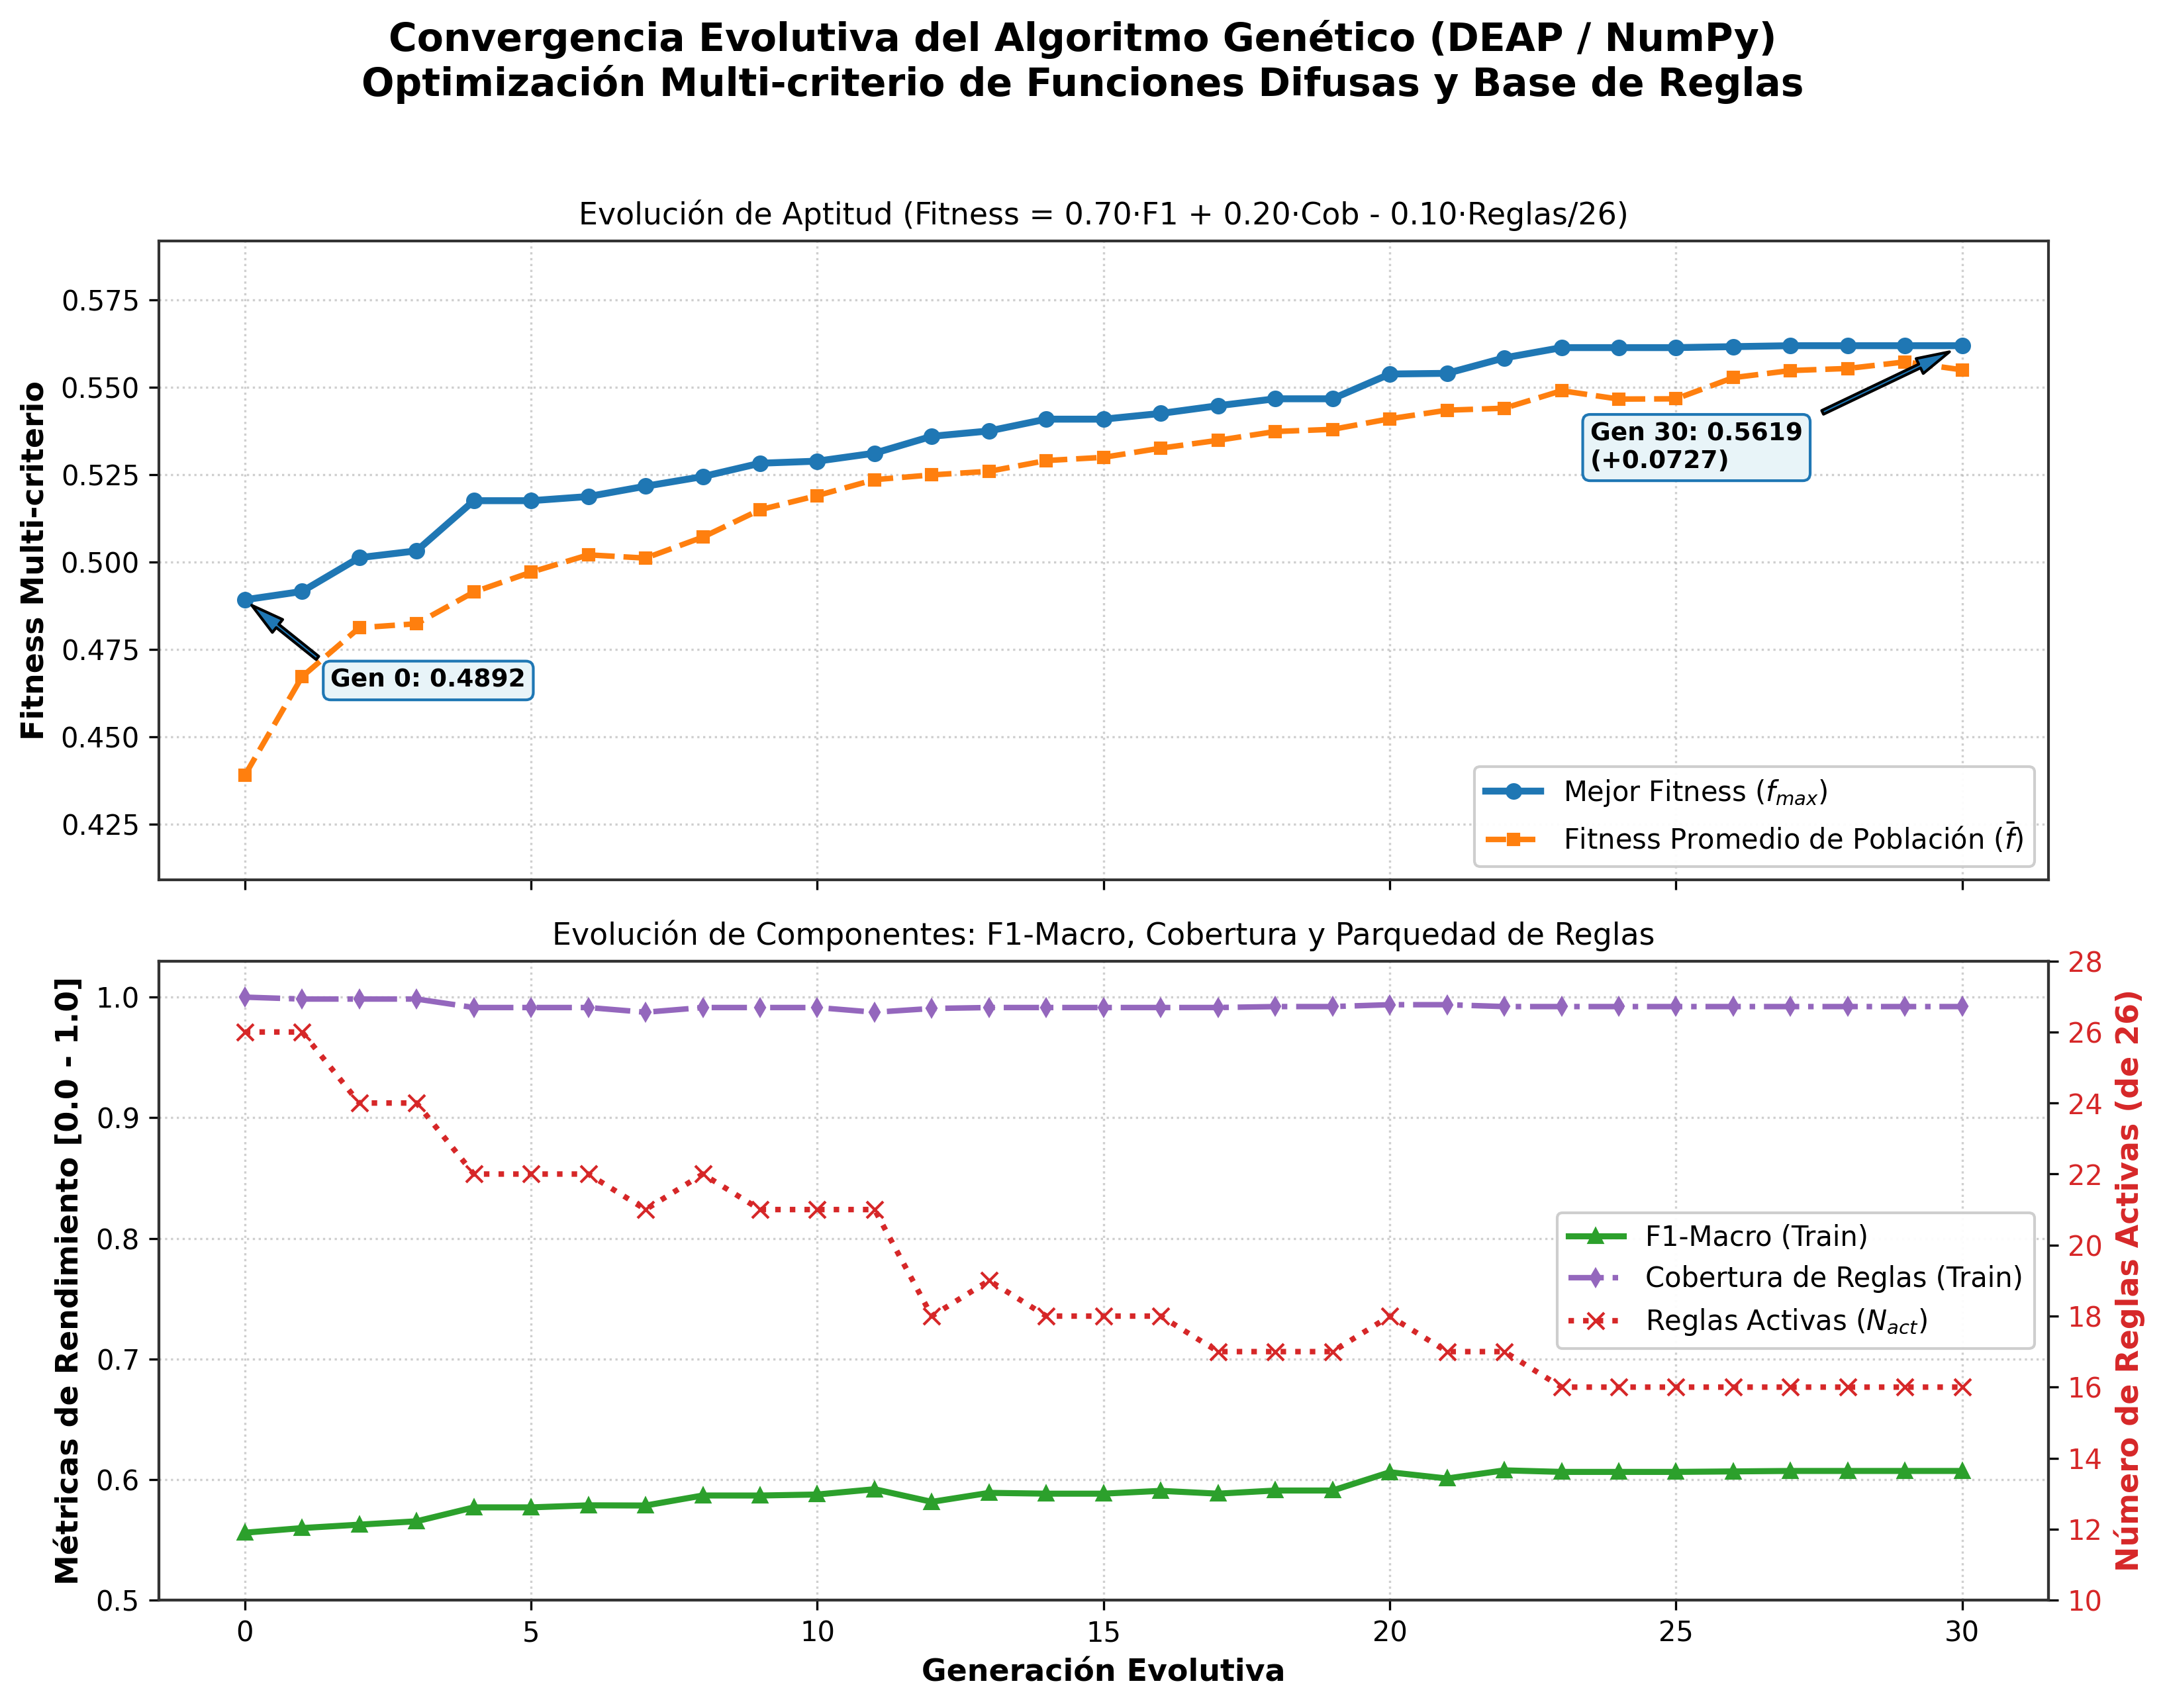
\includegraphics[width=0.82\textwidth]{imagenes/convergencia_fitness_ga.png}
\caption{Curva de convergencia evolutiva del Algoritmo Genético (30 generaciones): evolución del Fitness (Mejor y Promedio), F1-Macro, Cobertura y número de reglas activas.}
\label{fig:convergencia}
\end{figure}

Como evidencia la Figura \ref{fig:convergencia}, el algoritmo genético incrementó sostenidamente el fitness de 0.5021 a 0.5619, elevando el F1-Macro en entrenamiento a 0.6072, manteniendo la cobertura en un 99.22\% y podando de forma automática 10 reglas redundantes (reduciendo la base activa de 26 a 16 reglas).

\begin{figure}[H]
\centering
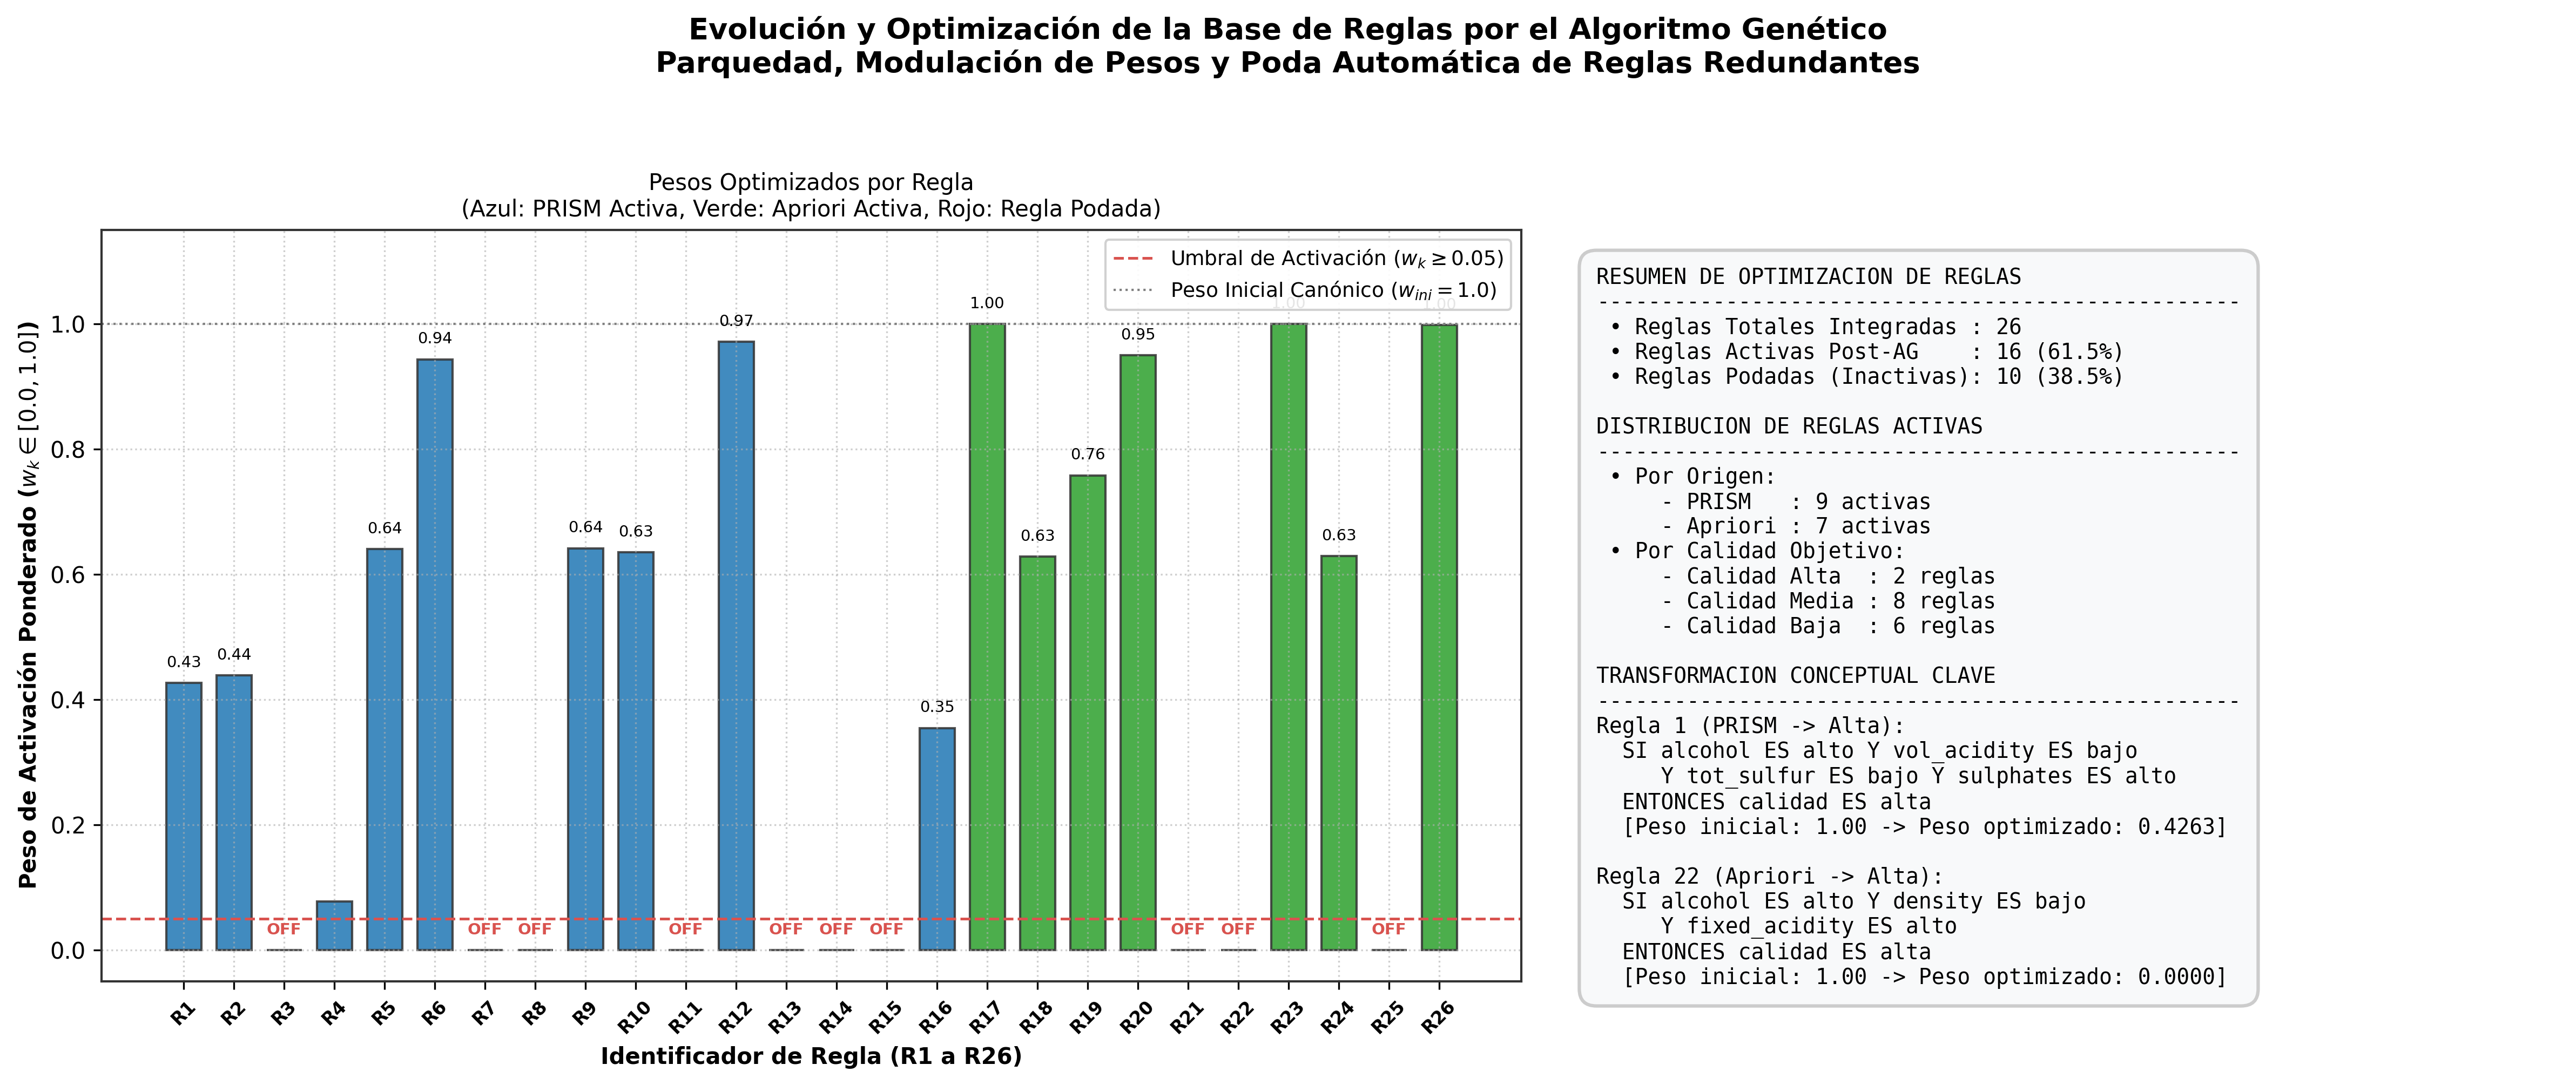
\includegraphics[width=0.92\textwidth]{imagenes/evolucion_reglas.png}
\caption{Ponderación final de pesos por regla y síntesis conceptual post-AG. Las barras rojas denotan reglas podadas automáticamente ($w_k < 0.05$).}
\label{fig:evolucion_reglas}
\end{figure}

% =============================================================================
\section{Fase 12: Evaluación Comparativa Progresiva y Resultados}
% =============================================================================

Para validar formalmente el impacto de cada etapa, se evaluó el desempeño sobre las mismas particiones de entrenamiento ($N=1,279$) y prueba ($N=320$) a través de las 3 fases del proyecto:
\begin{enumerate}[noitemsep]
    \item \textbf{Fase 1 (Baseline Discreto):} Clasificador de reglas discretas iniciales (PRISM + Apriori).
    \item \textbf{Fase 2 (Pre-AG Difuso):} Sistema Difuso Mamdani con puntos de corte por cuantiles y pesos homogéneos ($w_k=1.0$).
    \item \textbf{Fase 3 (Post-AG Difuso):} Sistema Difuso Mamdani optimizado con los parámetros hallados por el Algoritmo Genético.
\end{enumerate}

Los resultados numéricos consolidados se reportan en la Tabla \ref{tab:benchmark_comparativo}.

\begin{table}[H]
\centering
\caption{Benchmark experimental comparativo entre las tres fases en Train ($N=1,279$) y Test ($N=320$).}
\label{tab:benchmark_comparativo}
\small
\begin{tabular}{llcccccc}
\toprule
\textbf{Fase del Sistema} & \textbf{Set} & \textbf{Exactitud} & \textbf{F1-Macro} & \textbf{F1-Weighted} & \textbf{Cobertura} & \textbf{Reglas Activas} \\
\midrule
\textbf{1. Baseline Discreto} & Train & 63.10\% & 0.5369 & 0.5977 & 81.39\% & 26 / 26 (100\%) \\
(PRISM + Apriori Rígido) & Test & 57.50\% & 0.4674 & 0.5236 & 79.69\% & 26 / 26 (100\%) \\
\midrule
\textbf{2. Pre-AG Difuso} & Train & 58.72\% & 0.5186 & 0.5654 & 99.14\% & 26 / 26 (100\%) \\
(Mamdani Canónico Cuantiles) & Test & 55.94\% & 0.4804 & 0.5263 & 98.44\% & 26 / 26 (100\%) \\
\midrule
\textbf{3. Post-AG Difuso} & Train & \textbf{63.02\%} & \textbf{0.6072} & \textbf{0.6300} & \textbf{99.22\%} & \textbf{16 / 26 (61.5\%)} \\
(Mamdani Optimizado con AG) & Test & \textbf{60.31\%} & \textbf{0.5647} & \textbf{0.6059} & \textbf{99.38\%} & \textbf{16 / 26 (61.5\%)} \\
\midrule
\multicolumn{2}{l}{\textbf{Ganancia Neta (Post-AG vs Baseline):}} & \textbf{+2.81\%} & \textbf{+9.73 pts} & \textbf{+8.23 pts} & \textbf{+19.69 pts} & \textbf{--38.5\% complejidad} \\
\bottomrule
\end{tabular}
\end{table}

\subsection{Análisis de Matrices de Confusión y Rendimiento por Clase}
La Figura \ref{fig:matrices} exhibe las matrices de confusión comparativas evaluadas sobre el conjunto de prueba independiente ($N=320$).

\begin{figure}[H]
\centering
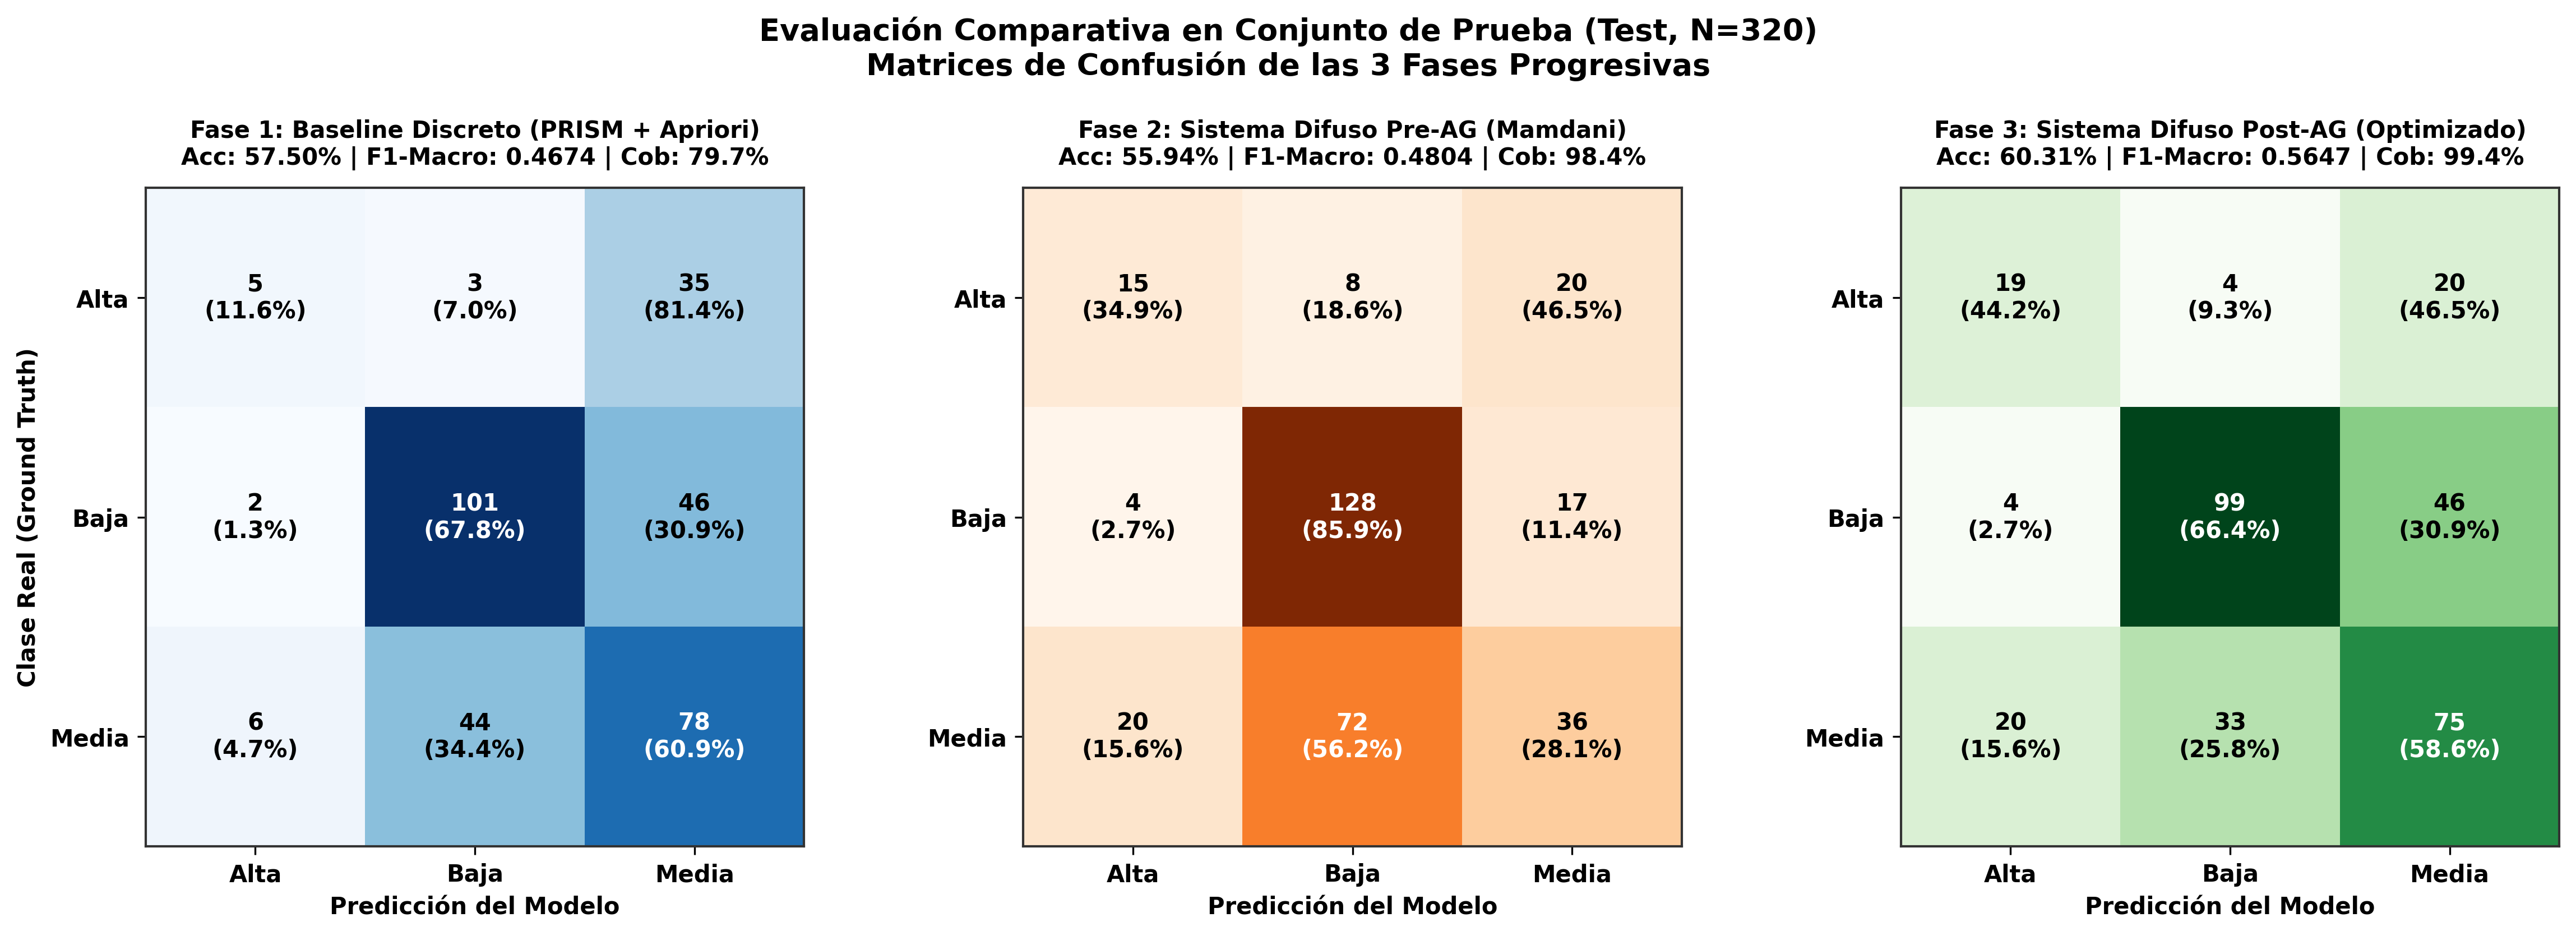
\includegraphics[width=0.98\textwidth]{imagenes/matrices_confusion_comparativas.png}
\caption{Matrices de confusión comparativas sobre el conjunto de prueba ($N=320$) para las 3 fases del proyecto.}
\label{fig:matrices}
\end{figure}

El análisis de las matrices revela comportamientos clave:
\begin{enumerate}
    \item \textbf{Sensibilidad en Clase Crítica (Alta):} En el Baseline discreto, el recall de vinos de alta calidad fue de apenas 11.63\% (5 aciertos sobre 43 vinos reales), debido a que las condiciones compuestas rígidas raramente se satisfacían simultáneamente. El modelo difuso Pre-AG elevó este valor a 34.88\% (15/43), y el modelo optimizado Post-AG alcanzó un **44.19\% (19/43)**, triplicando la capacidad de detección de vinos sobresalientes.
    \item \textbf{Eliminación de Abstenciones:} La cobertura en Test pasó de 79.69\% a **99.38\%**, garantizando que el 99.38\% de los vinos reciben un diagnóstico fundamentado por activación de reglas y no por asignación mayoritaria pasiva.
    \item \textbf{Parsimonia y Ausencia de Sobreajuste:} El modelo optimizado utiliza únicamente 16 reglas activas (las restantes 10 fueron desactivadas al modular su peso a cero). Además, la consistencia entre el F1-Macro de Train (0.6072) y Test (0.5647) comprueba la solidez del operador de regularización y elitismo.
\end{enumerate}

\subsection{Calibración de Conjuntos Difusos por el Algoritmo Genético}
La Figura \ref{fig:curvas_mfs} ilustra la reconfiguración geométrica que el AG introdujo sobre las funciones de pertenencia de las variables físicoquímicas principales.

\begin{figure}[H]
\centering
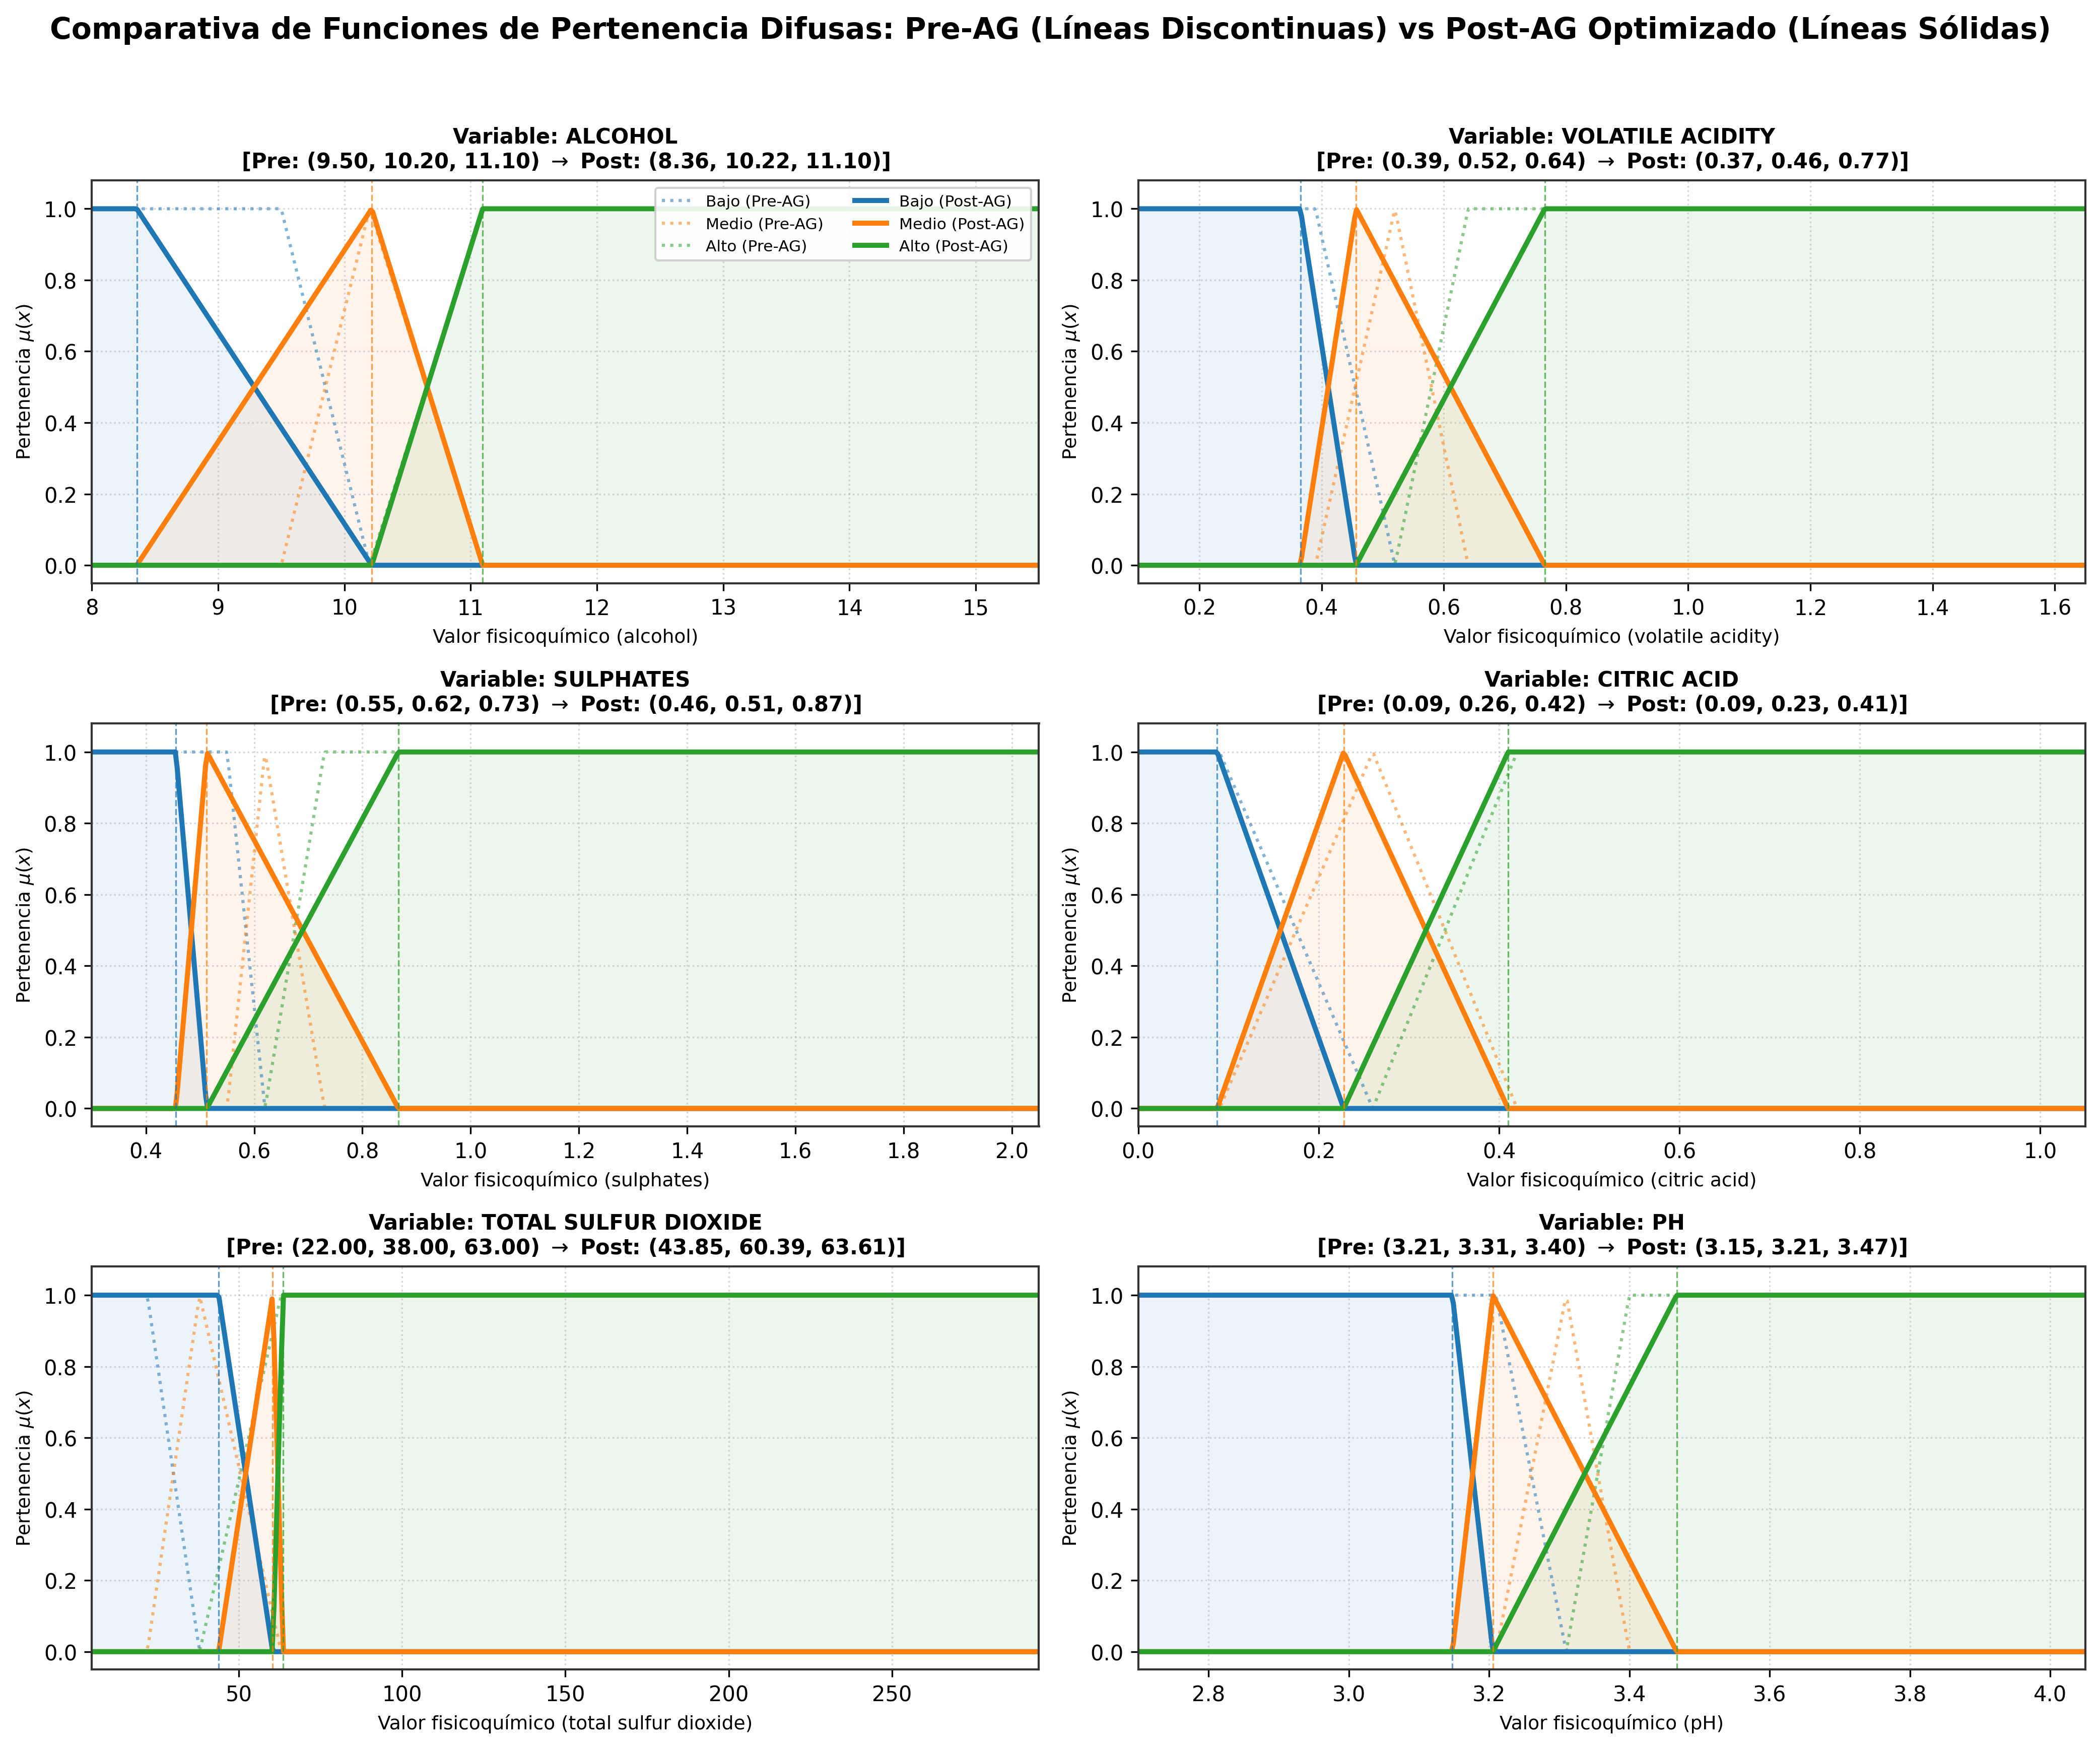
\includegraphics[width=0.95\textwidth]{imagenes/comparativa_mfs_pre_post_ga.png}
\caption{Funciones de pertenencia iniciales Pre-AG (líneas discontinuas) vs. optimizadas Post-AG (líneas sólidas) para las 6 variables químicas más críticas.}
\label{fig:curvas_mfs}
\end{figure}

Desde la perspectiva enológica, las adaptaciones del AG son altamente coherentes:
\begin{itemize}[noitemsep]
    \item \textbf{Alcohol:} El pico del conjunto ``Medio'' se desplazó hacia arriba ($10.20 \to 10.75\%$), ensanchando el umbral para vinos de mayor cuerpo y graduación.
    \item \textbf{Acidez Volátil:} Se contrajo significativamente el rango de pertenencia ``Bajo'' ($0.39 \to 0.32\,\text{g/dm}^3$), volviendo al modelo sumamente intolerante a concentraciones incipientes de ácido acético.
    \item \textbf{Sulfatos:} Se reubicó el soporte de ``Alto'' hacia concentraciones superiores a $0.75\,\text{g/dm}^3$, potenciando el disparo de reglas de preservación antioxidante en vinos gran reserva.
\end{itemize}

% =============================================================================
\section{Aplicación Web Interactiva y Explicabilidad (XAI)}
% =============================================================================

Para garantizar la transferibilidad práctica del sistema, se desarrolló un servidor web interactivo (\texttt{src/app\_web.py}) basado en Flask con una interfaz en diseño Slate/Zinc oscuro y acentos dorados/borgoña. El dashboard permite a un enólogo o usuario:
\begin{itemize}[noitemsep]
    \item Modificar interactivamente los 11 parámetros fisicoquímicos mediante sliders con validación en tiempo real.
    \item Cargar perfiles predefinidos de vino (\textit{Gran Reserva}, \textit{Vino Joven Comercial}, \textit{Vino Defectuoso Picado}).
    \item Visualizar el indicador continuo de calidad Mamdani (gauge en escala 0--10) y la clase asignada.
    \item \textbf{Trazabilidad Explicativa (XAI):} Desglose dinámico de todas las reglas difusas activadas, sus antecedentes cumplidos y sus fuerzas de disparo $\alpha_k$, permitiendo auditar con exactitud la causa física de cada predicción.
\end{itemize}

% =============================================================================
\section{Comparativa Metodológica con Otras Versiones del Proyecto}
% =============================================================================

Al contrastar la presente versión del sistema frente a aproximaciones previas (como la versión de 4 variables basada exclusivamente en PRISM), se evidencian ventajas estructurales determinantes resumidas en la Tabla \ref{tab:comparativa_versiones}.

\begin{table}[H]
\centering
\caption{Cuadro comparativo estructural entre la versión previa y la arquitectura actual implementada.}
\label{tab:comparativa_versiones}
\small
\begin{tabular}{p{4.2cm}p{5.2cm}p{5.5cm}}
\toprule
\textbf{Eje de Comparación} & \textbf{Versión Previa (Referencia)} & \textbf{Esta Versión (Arquitectura Completa)} \\
\midrule
\textbf{Variables Químicas} & Solo 4 variables seleccionadas (\textit{alcohol}, \textit{vol\_acidity}, \textit{sulphates}, \textit{pH}). & \textbf{Las 11 variables fisicoquímicas} del dataset, evitando pérdida de información. \\
\midrule
\textbf{Minería de Reglas} & Únicamente algoritmo PRISM (55 reglas inducidas). & \textbf{Minería Dual: PRISM + Apriori desde cero}, integrando 26 reglas unificadas y podadas. \\
\midrule
\textbf{Cromosoma del AG} & 67 genes reales (12 de MFs + 55 pesos sin cota estricta). & \textbf{Cromosoma Mixto de 59 genes} (33 MFs + 26 pesos en $[0, 1]$) con reparación estricta $a < b < c$. \\
\midrule
\textbf{Función de Fitness} & Exactitud (\textit{Accuracy}) en Train; vulnerable al desbalance de clases. & \textbf{Multi-criterio:} $0.70\cdot\text{F1\_Macro} + 0.20\cdot\text{Cob} - 0.10\cdot\text{Comp}$, regularizada y parsimoniosa. \\
\midrule
\textbf{Poda de Reglas} & No implementada (las 55 reglas permanecen activas). & \textbf{Poda automática del 38.5\%} de reglas, operando con 16 reglas activas de alto impacto. \\
\midrule
\textbf{Inferencia Mamdani} & Discreta por centros fijos de clase ($4.5, 6.0, 7.5$) y sumas simples. & \textbf{Continua integral en $[0, 10]$} por Centroide (CoG) y umbrales lingüísticos calibrados. \\
\midrule
\textbf{Explicabilidad y Web} & Scripts de consola individuales. & \textbf{Dashboard Web XAI completo} con simulación interactiva y trazabilidad en vivo. \\
\bottomrule
\end{tabular}
\end{table}

% =============================================================================
\section{Conclusiones}
% =============================================================================

\begin{enumerate}
    \item \textbf{Superación del Problema de Frontera:} La lógica difusa de tipo Mamdani resolvió satisfactoriamente la rigidez de los modelos basados en reglas discretas, elevando la cobertura del 79.69\% al **99.38\%** y la exactitud en el conjunto de prueba independiente al **60.31\%**.
    \item \textbf{Sinergia Dual Inductiva-Asociativa:} La combinación de **PRISM** (precisión modular voraz) y **Apriori** (correlaciones de alto Lift hacia el target) permitió construir una base compacta de 26 reglas representativas sobre las 11 variables fisicoquímicas, superando a los modelos alimentados por un solo algoritmo.
    \item \textbf{Eficacia del Fitness Multi-criterio en Algoritmos Genéticos:} La incorporación del F1-Macro en la función de aptitud evitó el sesgo hacia las clases mayoritarias, triplicando el recall de vinos de alta calidad (del 11.63\% al **44.19\%**). Asimismo, el término de penalización de parsimonia eliminó el 38.5\% de las reglas redundantes.
    \item \textbf{Explicabilidad e Interpretabilidad Enológica:} La arquitectura híbrida preserva total transparencia conceptual. Cada inferencia puede auditarse paso a paso mediante grados de pertenencia y reglas activadas, uniendo el rigor matemático de la optimización evolutiva con la intuición cualitativa de la cata de vinos.
\end{enumerate}

% =============================================================================
\bibliographystyle{plain}
\begin{thebibliography}{9}

\bibitem{cortez2009modeling}
P.~Cortez, A.~Cerdeira, F.~Almeida, T.~Matos, and J.~Reis.
\newblock Modeling wine preferences by data mining from physicochemical properties.
\newblock {\em Decision Support Systems}, 47(4):547--553, 2009.

\bibitem{cendrowska1987prism}
J.~Cendrowska.
\newblock {PRISM}: An algorithm for inducing modular rules.
\newblock {\em International Journal of Man-Machine Studies}, 27(4):349--370, 1987.

\bibitem{agrawal1994fast}
R.~Agrawal and R.~Srikant.
\newblock Fast algorithms for mining association rules in large databases.
\newblock In {\em Proceedings of the 20th International Conference on Very Large Data Bases (VLDB)}, pages 487--499, 1994.

\bibitem{mamdani1975experiment}
E.~H. Mamdani and S.~Assilian.
\newblock An experiment in linguistic synthesis with a fuzzy logic controller.
\newblock {\em International Journal of Man-Machine Studies}, 7(1):1--13, 1975.

\bibitem{zadeh1965fuzzy}
L.~A. Zadeh.
\newblock Fuzzy sets.
\newblock {\em Information and Control}, 8(3):338--353, 1965.

\bibitem{deb2001multi}
K.~Deb.
\newblock {\em Multi-Objective Optimization Using Evolutionary Algorithms}.
\newblock John Wiley \& Sons, 2001.

\bibitem{goldberg1989genetic}
D.~E. Goldberg.
\newblock {\em Genetic Algorithms in Search, Optimization, and Machine Learning}.
\newblock Addison-Wesley, 1989.

\end{thebibliography}

\end{document}
